
\chapter{Satellite Attitude Modeling}
\label{chap:SatelliteAttitudeModeling}

This chapter will cover the analytical work behind in this thesis.  Starting with the choice of attitude and body rate representations in Section \ref{sec:StateRepresentation} and how the application was written to incorporate its use.  Next, a review of some of the estimation-based control methods used including variations on their use to target their use on spin stabilized satellites such as NASA's MMS mission.  Then a summary of simulations run to validate the analytical model along with new tools used to visualize the system in ``run-time''.  Finally, testing of the analytical model against the physical system.

\section{State Representation}
\label{sec:StateRepresentation}

To represent the general state of a spin stabilized satellite, are often accomplished using one of two representations.  Either body rates with Euler angles or body rates with quaternions with Euler angles being slightly more common among control theory specialists and quaternions used more in the implementation of the control systems.  Euler angles with rigid body dynamics and quaternions were chosen for the state representation.  Quaternions provided unique advantages over Euler angles that will be expanded on in Sections \ref{subsec:BodyRate} and \ref{subsec:QuaternionAttitude}.

\subsection{Body Rates}
\label{subsec:BodyRate}

NASA's MMS satellites as with all real systems are rarely linear.  When modeling the dynamics of a system with nonlinearities, a common first pass is to linearize the model and assume that the nonlinearities are either negligible or can be lumped in to system disturbances.  This approach was also taken here.  The two portions of the system's dynamics are loosely generalized into either the rigid body dynamics of the satellite's main or the flexible dynamics of the attached booms.  Kaplan \cite{kaplan} covers the creation of the rigid body Euler's moment equations.

\begin{subequations}
  \begin{align}
    M_x = \dot{h}_x + \omega_y h_z - \omega_z h_y \\
    M_y = \dot{h}_y + \omega_z h_x - \omega_x h_z \\
    M_z = \dot{h}_z + \omega_x h_y - \omega_y h_x
  \end{align}
  \label{eqn:EulerMoment}
\end{subequations}

Here the equations of motion are described in terms of the body's frame of reference ($x$, $y$, $z$) which does not necessarily align with the body's principal axes.  TableSat 1A's construction can be simplified to an axisymmetric design.  To adjust TableSat 1A's stability, the center screw can be raised or lowered bringing the center of mass and center of rotation closer or further apart.  As development of the observer-based controller improves the two centers can be brought closer together.  With these conditions, we can assume that the body's reference frame aligns with the body's principal axes, which simplifies Euler's equations further to.

\begin{subequations}
  \begin{align}
    M_1 & = I_1 \dot{\omega}_1 + \omega_2 \omega_3 (I_3 - I_2) \\
    M_2 & = I_2 \dot{\omega}_2 + \omega_1 \omega_3 (I_1 - I_3) \\
    M_3 & = I_3 \dot{\omega}_3 + \omega_1 \omega_2 (I_2 - I_1)
  \end{align}
  \label{eqn:EulerMomentPrincipleAxes}
\end{subequations}

For implementation into the TableSat 1A's base station observer based controller, the continuous time Euler's equations \ref{eqn:EulerMomentPrincipleAxes} get converted to discrete time with a variable time step and implemented in Appendix \ref{code:TSatPy/State.py} as

\begin{subequations}
  \begin{align}
    \dot{\omega}_{x}(t_{k+1}) & = \frac{1}{I_x} \left[ M_1(t_{k+1}) - (I_z - I_y) \omega_{y}(t_k) \omega_{z}(t_k) \right] \\
    \dot{\omega}_{y}(t_{k+1}) & = \frac{1}{I_y} \left[ M_2(t_{k+1}) - (I_x - I_z) \omega_{x}(t_k) \omega_{z}(t_k) \right] \\
    \dot{\omega}_{z}(t_{k+1}) & = \frac{1}{I_z} \left[ M_3(t_{k+1}) - (I_y - I_x) \omega_{x}(t_k) \omega_{y}(t_k) \right]
  \end{align}
  \label{eqn:DiscreteEulerMomentEquations}
\end{subequations}

The moments $M_n(t_{k+1})$ are the applied moments at time $t_{k+1}$.  Since the update frequencies are allowed to vary for each section of the observer-based controller, the applied moment values may have multiple values between $t_{k}$ and $t_{k+1}$.  To avoid the complexity of calculating a more accurate moment for each time step that is a combination of changes in applied moments, the value of the most recent moments is taken and assumed constant for $t_{k} < t < t_{k+1}$.  If the moment update loop is running slower than the Euler equation model, the last known moment is assumed to still be valid.

While the Euler equation model works well for propagating the state of the system's, Section \ref{sec:Sensors} found that the only sources of state measurement were in attitude leaving body rates unmeasured.  Body rates must then be calculated through both observing changes in current attitude and state predictions based on previous attitude changes.  Euler angles and quaternions were investigated for parameterizing TableSat's attitude.

Euler angles were first considered because of their wide use in control theory where the representation of a body's attitude can be reached through a series of no more than three roll, pitch, yaw rotations.   Out of the twelve possible sequences, the 3-1-3 sequence is commonly used in spacecraft ADCS.  With this sequence Kaplan \cite{kaplan}, shows that the conversion between Euler angle rates and body rates can be calculated with

\begin{equation}
  \begin{bmatrix}
    \omega_x \\
    \omega_y \\
    \omega_z \\
  \end{bmatrix}
  =
  \begin{bmatrix}
    \sin \theta \sin \phi & \cos \phi & 0 \\
    \sin \theta \cos \phi & - \sin \phi & 0 \\
    \cos \theta & 0 & 1 \\
  \end{bmatrix}
  \begin{bmatrix}
    \dot{\psi} \\
    \dot{\theta} \\
    \dot{\phi} \\
  \end{bmatrix}
  \label{eqn:EulerToBodyRate}
\end{equation}

Euler angles while widely used and for most people easier to visualize, they have two main deficiencies.  They are heavily reliant on trigonometric functions and under certain conditions can cause singularities as seen by transforming Equation \ref{eqn:EulerToBodyRate} to solve for the Euler rates where a $1/\sin \theta$ factors out (Equation \ref{eqn:BodyRateToEuler}.  This phenomenon is more generally known as gimbal lock.  The second deficiency occurs in implementation, where the efficiency and stability of the angles are tied to the accuracy of trigonometric approximations in the code's library.  These repeated approximations are more prone to numerical drift.

\begin{equation}
  \begin{bmatrix}
    \dot{\psi} \\
    \dot{\theta} \\
    \dot{\phi} \\
  \end{bmatrix}
  =
  \frac{1}{\sin \theta}
  \begin{bmatrix}
    \sin \phi & \cos \phi & 0 \\
    \cos \phi \sin \theta & -\sin \phi \sin \theta & 0 \\
    -\sin \phi \cos \theta & -\cos \phi \cos \theta & \sin \theta \\
  \end{bmatrix}
  \begin{bmatrix}
    \omega_x \\
    \omega_y \\
    \omega_z \\
  \end{bmatrix}
  \label{eqn:BodyRateToEuler}
\end{equation}

The alternative attitude parameterization investigated was the quaternion attitude representation the conversion from body discrete body rates to quaternion attitude is calculated via the method from Trawny and Roumeliotis at the University of Minnesota \cite{marslab}.

\begin{equation}
  \begin{aligned}
    \bs{q}(t_{k+1}) = & \bigg[ \exp \left( \frac{\Delta t_{k+1}}{2} \bs{\Omega} \left[ \bs{\bar{\omega}}(t_{k+1}) \right] \right) + \\
    & \frac{1}{48} \Delta t_{k+1}^2 \Big(
    \bs{\Omega} \left[\bs{\omega}(t_{k+1}) \right]
    \bs{\Omega} \left[\bs{\omega}(t_{k})   \right] -
    \bs{\Omega} \left[\bs{\omega}(t_{k})   \right]
    \bs{\Omega} \left[\bs{\omega}(t_{k+1}) \right]
      \Big) \bigg] \bs{q}(t_{k})
  \end{aligned}
  \label{eqn:DiscreteQuaternionPropagation}
\end{equation}

where

\begin{equation}
    \bs{\Omega} \left[ \bs{\bar{\omega}}(t_{k+1}) \right] = \frac{\bs{\Omega} \left[\bs{\omega}(t_{k+1}) \right] + \bs{\Omega} \left[\bs{\omega}(t_{k}) \right]}{2}
    \label{eqn:DiscreteQuaternionToBodyRate}
\end{equation}

\begin{equation}
  \bs{\Omega} \left[ \bs{\omega} \right] =
  \begin{bmatrix}
    - [ \bs{\omega} \times ] & \bs{\omega} \\
    - \bs{\omega}^T & 0 \\
  \end{bmatrix}
  \label{eqn:OmegaMatrix}
\end{equation}

\begin{equation}
  \bs{\omega} \times =
  \begin{bmatrix}
    0 & -\bs{\omega}_z & \bs{\omega}_y \\
    \bs{\omega}_z & 0 & -\bs{\omega}_x \\
    -\bs{\omega}_y & \bs{\omega}_x & 0 \\
  \end{bmatrix}
\end{equation}


\subsection{Quaternion Attitude}
\label{subsec:QuaternionAttitude}

The concept of a quaternion is a combination of geometry and algebra based focus from Rodrigues and Hamilton respectively \cite{shuster}.  Rodrigues' work in the early 1800's focused the Gibbs vector as a way of creating a an attitude matrix from the Rodrigues parameters.  Hamilton's work focused on hyper-complex numbers with three hyper-imaginary values and a constant.  Hamilton first coined the term quaternion in 1843 to describe the four dimensional vector.  The four orthogonal unit quaternions are

\begin{subequations}
  \begin{align}
    \bs{1} = & 1 + 0\bs{i} + 0\bs{j} + 0\bs{k} \\
    \bs{i} = & 0 + 1\bs{i} + 0\bs{j} + 0\bs{k} \\
    \bs{j} = & 0 + 0\bs{i} + 1\bs{j} + 0\bs{k} \\
    \bs{k} = & 0 + 0\bs{i} + 0\bs{j} + 1\bs{k}
  \end{align}
  \label{eqn:UnitQuaternions}
\end{subequations}

where the unit quaternions obey Hamilton's rules \cite{wolfram_quaternion}

\begin{subequations}
  \begin{align}
    \bs{i}^2 = \bs{j}^2 = \bs{k}^2 = \bs{ijk} & = - \bs{1} \\
    \bs{i}\bs{j} = -\bs{j}\bs{i} &= \bs{k} \\
    \bs{j}\bs{k} = -\bs{k}\bs{j} &= \bs{i} \\
    \bs{k}\bs{i} = -\bs{i}\bs{k} &= \bs{j}
  \end{align}
  \label{eqn:HamiltonRules}
\end{subequations}

As discussed in Section \ref{subsec:StateMeasurement}, between TableSat sensor and MMS mission restrictions, the body rate for this research is not measured.  This meant that the choice in attitude parameterization and how it is implemented play a major factor in the entire system's performance.  Because of their numerical stability and that over time I found working with quaternions more intuitive than Euler angles, the quaternion was chosen as the method for representing state attitude parameters.  From sections \TODO{label these later} to \TODO{XXX}, quaternion properties will be discussed along with how they were represented in the controller's implementation.

\subsubsection{Quaternion Notation}
\label{subsubsec:QuaternionNotation}

One point of confusion when working with quaternions is the placement of the scalar term.  As shown in Equation \ref{eqn:UnitQuaternions} the scalar term is followed by the three complex terms.  To stay consistent with related research, the quaternion notation to be used in this thesis follows the structure of 4 dimensional vector where the scalar term follows the vector.

\begin{equation}
  \bs{q} = \bs{v} + q_0 = q_1 \bs{i} + q_2 \bs{j} + q_3 \bs{k} + q_0
\end{equation}

In academic literature, the difference is not terribly significant as the notation is generally defined by the author or the reader can recognize the variation in structure.  For example in Equation \ref{eqn:OmegaMatrix}, written in a scalar last format, is composed from a 3x3, 3x1, 1x3, and 1x1.  During implementation, mixing of scalar first matrices with scalar last matrices can be a troublesome source of error.  As will be described more in Chapter \ref{chap:TSatPy}, the implementation in this thesis is done in an object oriented manner so it can handle either the scalar first or scalar last format.

\begin{singlespace}
  \begin{minted}[mathescape,linenos,numbersep=10pt,frame=lines,framesep=2mm]{python}
from TSatPy.State import Quaternion
q = Quaternion(vector=[1,2,3], scalar=4)
print(q)
q = Quaternion(scalar=0, vector=[1,2,3])
print(q)

# Prints Out
# <Quaternion [1 2 3], 4>
# <Quaternion [1 2 3], 0>
  \end{minted}
  \nocite{minted}
\end{singlespace}

\subsubsection{Rotational Quaternion}
\label{subsubsec:RotationalQuaternion}

Euler's rotation theorem states:

\begin{quote}{``\textsl{If $\bs{R}$ is a 3x3 orthogonal matrix $( \bs{R}^T \bs{R} = \bs{R}\bs{R}^T = \bs{I} )$ and $\bs{R}$ is proper $( det \bs{R} = +1 )$, then there is a nonzero vector $\bs{v}$ satisfying $\bs{Rv} = \bs{v}$}''~\cite{euler_theorem}}\end{quote}

With a 3x3 rotational matrix, this means there is a line of points that do not change position and create an axis of rotation.  Incorporating this idea into any spin stabilized satellite like NASA's MMS mission yields that any arbitrary attitude can be represented as a single rotation from a common starting orientation.  The axis $\hat{e}$ and the angle of rotation $\theta$ can express the satellite's attitude with a rotational quaternion as

\begin{equation}
  \bs{q} = \bs{v} + q_0 = \hat{\bs{e}} \sin \left( \frac{-\theta}{2} \right) + \cos \left( \frac{-\theta}{2} \right)
  \label{eqn:RotationalQuaternionDefinition}
\end{equation}

A $-\theta$ is used rather than a the positive value to represents points on the body frame rotating around fixed axes rather than an axes transformation.  This representation also reduces the degrees of freedom for a quaternion from four to three as a rotational quaternion is restricted to always having a unit norm.

\begin{equation}
  \left| \hat{\bs{e}} \sin \left( \frac{-\theta}{2} \right) + \cos \left( \frac{-\theta}{2} \right) \right| = \left| \hat{\bs{e}} \right|  \sin^2 \left( \frac{-\theta}{2} \right) + \cos^2 \left( \frac{-\theta}{2} \right) = 1
\end{equation}

Creating a rotational quaternion from the TSatPy (Chapter \ref{chap:TSatPy}) is done with

\begin{singlespace}
  \begin{minted}[mathescape,linenos,numbersep=10pt,frame=lines,framesep=2mm]{python}
from TSatPy.State import Quaternion

q = Quaternion(vector=[1,2,3], radians=4)
e, theta = q.to_rotation()

print(q)
print("Euler axis: <%g, %g, %g>" % (e[0,0], e[1,0], e[2,0]))
print("Rotation: %g radians" % theta)

# Prints Out
# <Quaternion [-0.24302 -0.48604 -0.72906], -0.416147>
# Euler axis: <-0.267261, -0.534522, -0.801784>
# Rotation: 4 radians
  \end{minted}
  \nocite{minted}
\end{singlespace}


\subsubsection{Quaternion Multiplication}
\label{subsubsec:QuaternionMultiplication}

The quaternion multiplication noted with the infix operator $\otimes$, is the keystone to the attitude state manipulation and is used to produce incremental changes in the satellite's attitude.  If $\bs{a}$ represents a $n$ degree rotation about axis $\hat{e}$, then a $4n$ degree rotation about axis $\hat{e}$ can be represented as $\bs{a} \otimes \bs{a} \otimes \bs{a} \otimes \bs{a}$.

The example below shows how this incremental changes holds true with the TSatPy library.

\begin{singlespace}
  \begin{minted}[mathescape,linenos,numbersep=10pt,frame=lines,framesep=2mm]{python}
from TSatPy.State import Quaternion

a = Quaternion([1,2,3], radians=0.5)
b = Quaternion([1,2,3], radians=2)
print("a             = %s" % a)
print("a * a * a * a = %s" % (a * a * a * a))
print("b             = %s" % b)
# Prints Out
# a             = <Quaternion [-0.0661215 -0.132243 -0.198364], 0.968912>
# a * a * a * a = <Quaternion [-0.224893 -0.449785 -0.674678], 0.540302>
# b             = <Quaternion [-0.224893 -0.449785 -0.674678], 0.540302>
  \end{minted}
  \nocite{minted}
\end{singlespace}

Let $\bs{a}$ and $\bs{b}$ represent two quaternions where

\begin{subequations}
\begin{align}
  \bs{a} = \bs{a}_v + a_0 = & a_1 \bs{i} + a_2 \bs{j} + a_3 \bs{k} + a_0\\
  \bs{b} = \bs{b}_v + b_0 = & b_1 \bs{i} + b_2 \bs{j} + b_3 \bs{k} + b_0
\end{align}
\end{subequations}

The quaternion multiplication is defined as

\begin{equation}
  \bs{q} = \bs{a} \otimes \bs{b} = \bs{a}_v b_0 + \bs{b}_v a_0 + \bs{a}_v \times \bs{b}_v + a_0 b_0 - \bs{a}_v \cdot \bs{b}_v
  \label{eqn:QuaternionMultiplication}
\end{equation}

Expanding Equation \ref{eqn:QuaternionMultiplication} yields

\begin{subequations}
\begin{align}
  \bs{v} & = \begin{bmatrix} a_1 \\ a_2 \\ a_3 \end{bmatrix} b_0 +\begin{bmatrix} b_1 \\ b_2 \\ b_3 \end{bmatrix} a_0 + \begin{bmatrix} a_1 \\ a_2 \\ a_3 \end{bmatrix} \times \begin{bmatrix} b_1 \\ b_2 \\ b_3 \end{bmatrix} \\
  q_0 & = a_0 b_0 - \bs{a}_v \cdot \bs{b}_v
\end{align}
\end{subequations}

Evaluating the cross and dot products

\begin{subequations}
\begin{align}
  \bs{v} & = \begin{bmatrix} a_1 \\ a_2 \\ a_3 \end{bmatrix} b_0 +\begin{bmatrix} b_1 \\ b_2 \\ b_3 \end{bmatrix} a_0 + \begin{bmatrix} a_2b_3 - a_3b_2 \\ a_3b_1 - a_1b_3 \\ a_1b_2 - a_2b_1 \\ \end{bmatrix} \\
  q_0 & = a_0 b_0 - (a_1b_1 + a_2b_2 + a_3b_3)
\end{align}
\end{subequations}

\begin{subequations}
\begin{align}
  \bs{v} & = \begin{bmatrix} a_1b_0 + b_1a_0 + a_2b_3 - a_3b_2 \\ a_2b_0 + b_2a_0 + a_3b_1 - a_1b_3 \\ a_3b_0 + b_3a_0 + a_1b_2 - a_2b_1 \\ \end{bmatrix} \\
  q_0 & = a_0 b_0 - a_1b_1 - a_2b_2 - a_3b_3
\end{align}
\end{subequations}

Combining equations and factoring out the $b$ terms yields

\begin{equation}
  \begin{bmatrix} \bs{v} \\ q_0 \end{bmatrix} =
  \begin{bmatrix}
    a_0 & - a_3 &   a_2 & a_1 \\
    a_3 &   a_0 & - a_1 & a_2 \\
  - a_2 &   a_1 &   a_0 & a_3 \\
  - a_1 & - a_2 & - a_3 & a_0
  \end{bmatrix}
  \begin{bmatrix}
  b_1 \\ b_2 \\ b_3 \\ b_0
  \end{bmatrix}
\end{equation}

From here, the square matrix can be decomposed into sections based on if they get combined with quaternion $b$'s vector or scalar components.  Once segmented, the components of the square matrix can be expressed more compactly and in a way that conveys a better sense of how the quaternions interact on multiplication.

\begin{equation}
  \begin{bmatrix} \bs{v} \\ q_0 \end{bmatrix} =
  \begin{bmatrix}
    (\bs{a}_v \times) + \bs{I} a_0 & \bs{a}_v \\
    -\bs{a}_v^T                    & a_0 \\
  \end{bmatrix}
  \begin{bmatrix}
  \bs{b}_v \\ b_0
  \end{bmatrix}
  \label{eqn:QuaternionMultiplicationDerived}
\end{equation}

This quaternion class for TSatPy as will be covered in Chapter \ref{chap:TSatPy} allows for the a very close representation of Equation \ref{eqn:QuaternionMultiplicationDerived}.  Section \ref{subsubsec:QuaternionMultiplication} includes a small example of quaternion multiplication and the following snippet is the implementation of the quaternion multiplication which reads and is used similarly to how the quaternion algebra is written.

\begin{singlespace}
  \begin{minted}[mathescape,linenos,numbersep=10pt,frame=lines,framesep=2mm]{python}
class Quaternion(object):
    def __mul__(self, q):
        v = (self.x + np.eye(3) * self.scalar) * q.vector
        v += self.vector * q.scalar
        s = self.scalar * q.scalar - (self.vector.T * q.vector)[0, 0]
        return Quaternion(v, s)
  \end{minted}
  \nocite{minted}
\end{singlespace}

\subsubsection{Rotating a Point with Quaternions}
\label{subsubsec:RotatingaPointwithQuaternions}

One of the main focal points of this thesis is to make sure the tools developed aide in outreach and demonstration.  To enable this goal, ``run-time'' analysis of the system is a key deliverable.  Waiting for a simulation to complete or a experimental run with TableSat before being able to access the information is not only an impedance to this end, but it also introduces complexity and higher ``run-time'' costs to collect and store the full history of the system for replay.  One advantage to having access to the system's parameters as the experiment proceeds is to be able to represent the inner workings of the algorithms for inspection.  In the case of an estimator, sensor voltages are converted to a measured state and the estimator attempts to guess the true state of the system.  A visualization of what the estimator thinks the TableSat is doing can run alongside the physical systems and the convergence between estimated and actual states can be readily observed.

To facilitate this, visualization a model of the TableSat can be rotated with a rotation matrix based on the estimated state's quaternion.  The 3x3 rotation matrix is defined as a function of a rotational quaternion by

\begin{equation}
  \bs{R_q} = (q_0^2 - \bs{v}^T \bs{v}) \bs{I} + 2 \bs{v} \bs{v}^T - 2 q_0 (\bs{v} \times)
  \label{eqn:RotationMatrix}
\end{equation}

For a $\pi/2$ radian rotation about $\hat{e} = 0\bs{i}+0\bs{j}+1\bs{k}$, the rotational quaternion an defined in Equation \ref{eqn:RotationalQuaternionDefinition} becomes $q = 0\bs{i}+0\bs{j}-1/\sqrt{2}\bs{k}+1/\sqrt{2}$.  With Equation \ref{eqn:RotationMatrix}, the rotational matrix becomes

\begin{equation}
  \begin{aligned}
    \bs{R_q} & = \left[ (1/\sqrt{2})^2 - (1/\sqrt{2})^2 \right] \bs{I} + 2 \begin{bmatrix} 0 & 0 & 0 \\ 0 & 0 & 0 \\ 0 & 0 & 1/\sqrt{2} \end{bmatrix} - 2 \frac{1}{\sqrt{2}} \begin{bmatrix} 0 & 1/\sqrt{2} & 0 \\ -1/\sqrt{2} & 0 & 0 \\ 0 & 0 & 0 \\ \end{bmatrix} \\
      & = \begin{bmatrix} 0 & -1 & 0 \\ 1 & 0 & 0 \\ 0 & 0 & 1 \\\end{bmatrix}
  \end{aligned}
\end{equation}

For the visualization, a point $A (2, 4, -1)$ that in the standard orientation of body axes aligned with the global reference frame can be drawn at the current estimated location of

\begin{equation}
  A' = \bs{R_q} A = \begin{bmatrix} 0 & -1 & 0 \\ 1 & 0 & 0 \\ 0 & 0 & 1 \\\end{bmatrix} \begin{bmatrix} 2 \\ 4 \\ -1 \end{bmatrix} = \begin{bmatrix} -4 \\ 2 \\ -1 \end{bmatrix}
\end{equation}

The equivalent TSatPy implementation of this point rotation is

\begin{singlespace}
  \begin{minted}[mathescape,linenos,numbersep=10pt,frame=lines,framesep=2mm]{python}
from TSatPy.State import Quaternion
import numpy as np

A = np.mat([2, 4, -1]).T
q = Quaternion([0,0,1], radians=np.pi/2)

print(q.rmatrix * A)

# Prints out
# [[-4.]
#  [ 2.]
#  [-1.]]
  \end{minted}
  \nocite{minted}
\end{singlespace}


\subsubsection{Quaternion-based Attitude Visualization}
\label{subsubsec:QuaternionbasedAttitudeVisualization}

Now that we have a method for calculating the new position of a point from an initial position, we can extend the process to a collection of points that create a wireframe for the TableSat model.  Once this base wireframe is defined, the estimated attitude of the system can be visualized.  The if the system's estimator determines that TableSat is at an attitude of $\bs{q} = -0.38\bs{i}-0.07\bs{j}+0.91\bs{k}+0.16$, that is equivalent to a 161 degree rotation about the axis $\bs{\hat{e}} = <0.38, 0.07, -0.92>$.  Figure \ref{fig:TSatWireframe} shows the TableSat wireframe in its default configuration with body axes align with the global reference frame.  The red dashed line shown is the axis of rotation.

\begin{figure}[H]
  \centerline{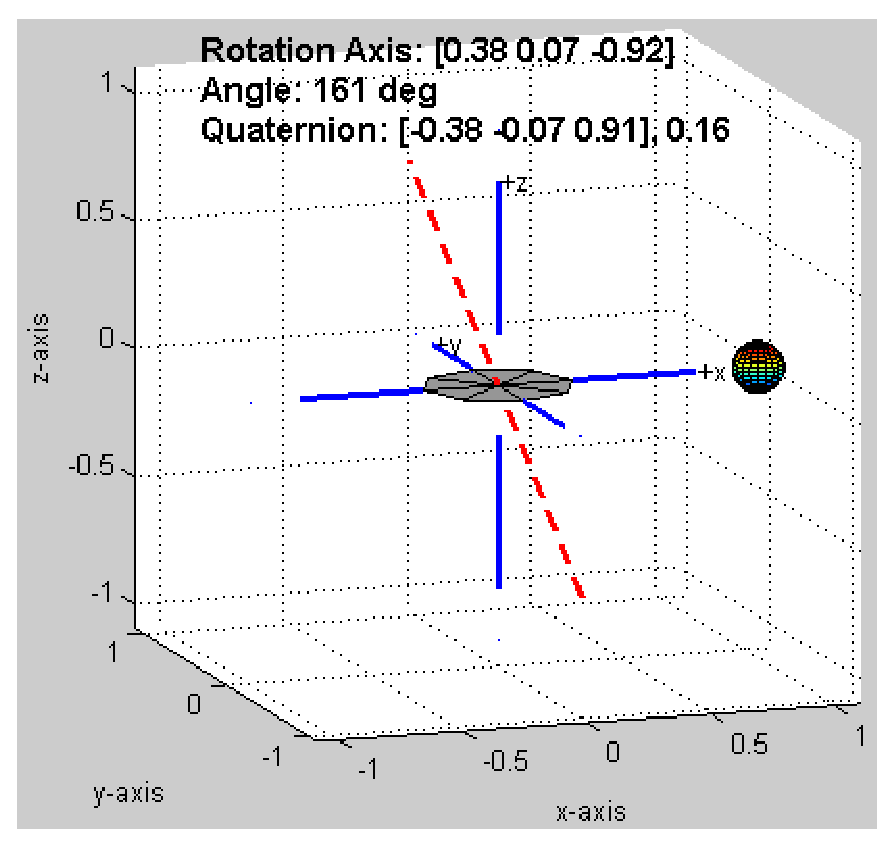
\psfig{file=figures/q_rotation_start.eps,height=3in}}
  \caption{TableSat Wireframe}
  \label{fig:TSatWireframe}
\end{figure}

The collection of the points in the TableSat wireframe can be rotated as the single point was from above.  Once new locations are determined, the TableSat wireframe can be redrawn visualizing the estimated current orientation of the TableSat (Figure \ref{fig:TSatWireframeEstimatedAttitude}).  Chapter \ref{chap:SoftwareDevelopmentforExperimentalIntegration} will cover the ``run-time'' visualizations in greater detail to show how as the estimator is running, updates to the estimated state, $\bs{\hat{x}}$, can be used to update the wireframe's orientation.

\begin{figure}[H]
  \centerline{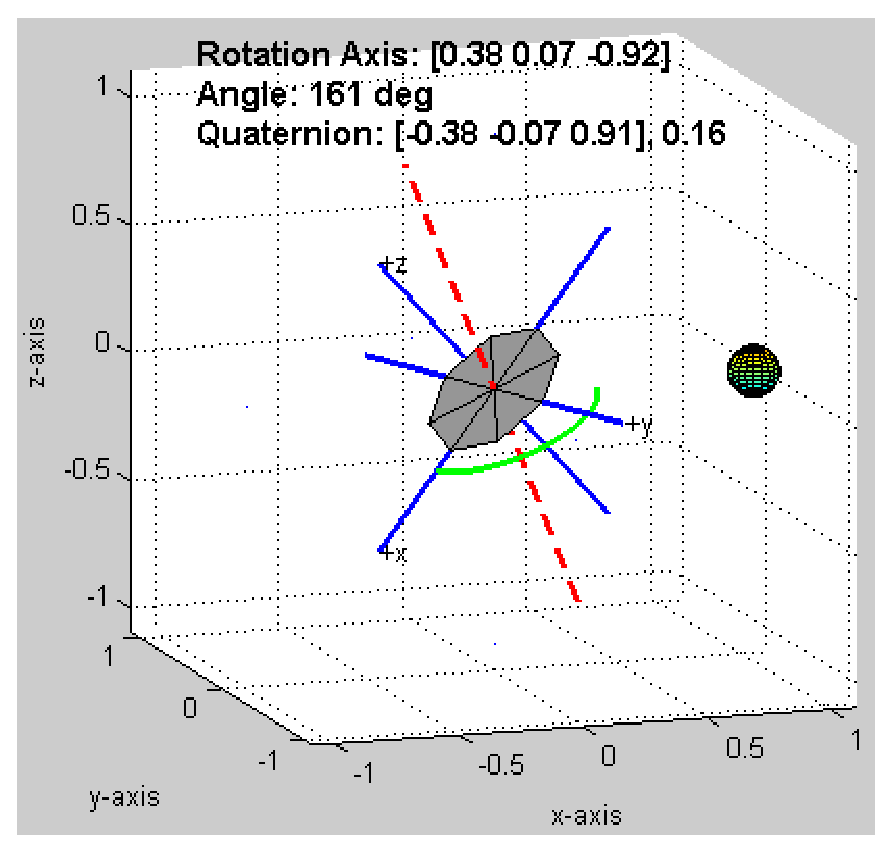
\psfig{file=figures/q_rotation_end.eps,height=3in}}
  \caption{TableSat Wireframe Estimated Attitude}
  \label{fig:TSatWireframeEstimatedAttitude}
\end{figure}


\subsubsection{Incremental Rotations}
\label{subsubsec:IncrementalRotations}

The quaternion's definition based on Euler's theorem of a rotation about a single axis makes tracking the orientation of a spin stabilized satellite an easier process.  NASA's MMS mission has a target spin rate of 3 rpm (~0.314 rad/sec).  A rotational quaternion representing the per second rotation about the z-axis is

\begin{equation}
  \begin{aligned}
    \bs{q}_{rps} = & ( 0\bs{i} + 0\bs{j} + 1\bs{k} ) \sin \left( \frac{-0.314}{2} \right) + \cos \left( \frac{-0.314}{2} \right) \\
    = & 0\bs{i} +0\bs{j} -0.156434\bs{k} + 0.987688
  \end{aligned}
\end{equation}

In an open loop system, the best estimate of the systems state would be to apply the quaternion rotation each second to the previous steps state starting with an initially known orientation.  For example if we have the TableSat at a $+1/4$ turn about the z-axis, each second we can calculate the best guess at the current attitude using just a quaternion multiplication.

\begin{equation}
  \begin{aligned}
    \bs{q}(t_{k+1}) = & \bs{q}_{rps} \otimes \bs{q}(t_{k}) \\
    \text{where } \bs{q}(t_0) = & 0 \bs{i} +0 \bs{j} -0.707107 \bs{k} +0.707107
  \end{aligned}
  \label{eqn:3rpmQuaternionEquation}
\end{equation}

Using the TSatPy code, equation \ref{eqn:3rpmQuaternionEquation} can be implemented as

\begin{singlespace}
  \begin{minted}[mathescape,linenos,numbersep=10pt,frame=lines,framesep=2mm]{python}
from TSatPy.State import Quaternion
import time
import numpy as np

q_rps = Quaternion([0,0,1], radians=np.pi/10)
print('Quaternion spin rate (rad/sec)\n %s' % q_rps)

q_state = Quaternion([0,0,1], radians=np.pi/2)
print('Initial state of TableSat\n t=0: %s' % q_state)


print('Starting Open Loop State Tracking')
for k in range(1,11):
    time.sleep(1)
    q_state *= q_rps
    print(' t=%s: %s' % (k, q_state))

# Prints Out
# Quaternion spin rate (rad/sec)
#  <Quaternion [-0 -0 -0.156434], 0.987688>
# Initial state of TableSat
#  t=0: <Quaternion [-0 -0 -0.707107], 0.707107>
# Starting Open Loop State Tracking
#  t=1: <Quaternion [0 0 -0.809017], 0.587785>
#  t=2: <Quaternion [0 0 -0.891007], 0.45399>
#  t=3: <Quaternion [0 0 -0.951057], 0.309017>
#  t=4: <Quaternion [0 0 -0.987688], 0.156434>
#  t=5: <Quaternion [0 0 -1], 1.11022e-16>
#  t=6: <Quaternion [0 0 -0.987688], -0.156434>
#  t=7: <Quaternion [0 0 -0.951057], -0.309017>
#  t=8: <Quaternion [0 0 -0.891007], -0.45399>
#  t=9: <Quaternion [0 0 -0.809017], -0.587785>
#  t=10: <Quaternion [0 0 -0.707107], -0.707107>
  \end{minted}
  \nocite{minted}
\end{singlespace}

This implementation has both a big control theory and implementation issue.  The control theory concern is the estimate is running in an open loop without ever receiving corrections so the myriad of additional factors that affect a real system would quickly invalidate the accuracy of the estimate in this approach.  The implementation issue deals with the time step.  Even if TableSat/MMS spun perfectly at 3 rpm the state will not be updated exactly on each second.  A busy processor, numerical drift, and execution time will prevent the desired fixed step size of 1 sec.  In some of the earlier implementations of the base station controller discussed in Chapter \ref{chap:StandardTools} dropped UDP messages caused the control loop to execute on an inconsistent interval and prevent accurate state estimates.  Handling of the variability in timesteps will be covered Section \ref{sec:SatelliteDynamics}

\section{Satellite Dynamics}
\label{sec:SatelliteDynamics}

The goal in creating an accurate satellite dynamics model is it's ability to predict the state of the system given the last know state, the elapsed time since the last known state, and any inputs or disturbances to the system.  The initial scope of predicting the satellite's state is restricting it to a state propagation problem where only last state and elapsed time are considered.  Estimation techniques in Section \ref{sec:Estimators} will cover how a propagated state can be adjusted using the measured state.

\subsection{System Clock}
\label{subsec:SystemClock}

As was mentioned at the end of section \ref{subsubsec:IncrementalRotations}, perfectly timed updates are highly unlikely.  Small variations in the timestep size will cause predicted state errors.  A state update running every 1.0001 seconds instead of every second would accumulate over a six degree error after tracking TableSat's state for an hour.  Linearized model would also be affected because the expected timestep size is incorporated as part of the discretization processes.

The preset fixed timestep is also not very fault tolerant.  When controlling the state of a stable, slow moving system the state tracking rate could be slowed down to conserve system resources.  In this circumstance a missed or series of missed updates due to faults can cause the predicted state to be several $\Delta t$ behind where it should be.  A solution built for variable steps can improve the robustness against these errors.

The ability to slow down a simulation to closely watch the initial transient behavior followed speeding up the simulation to inspect long term stability hold benefits for both outreach and research purposes.  The TSatPy system was built with this idea in mind which addresses the previous two issues as the system by design needs to be able to smoothly transition between variations in step sizes in a single run.


\begin{equation}
  \begin{aligned}
    t_k =& \sum\limits_{i=0}^{k-1} r_i (\tau_{i+1} - \tau_i)\\
    \text{where } \tau =& \text{ real time} \\
    t_k =& \text{ simulation time at step }k
  \end{aligned}
  \label{eqn:SystemTime}
\end{equation}

The system clock defined in Equation \ref{eqn:SystemTime} starts at zero and accumulates time depending on the set rate.  TSatPy implements this concept through the Metronome class.  An instance of this class serves as the reference frame for all rate calculations.  During the simulation, the clock is able to slow and quicken based on the set speed.

\begin{singlespace}
  \begin{minted}[mathescape,linenos,numbersep=10pt,frame=lines,framesep=2mm]{python}
from TSatPy.Clock import Metronome
import time

c = Metronome()
print("Start Time: system=%s, real=%s" % (c, time.time()))
time.sleep(2)
print("Lock step:  system=%s, real=%s" % (c, time.time()))
c.set_speed(0.1)
time.sleep(30)
print("Slow-mo:    system=%s, real=%s" % (c, time.time()))
c.set_speed(100)
time.sleep(4)
print("FFW:        system=%s, real=%s" % (c, time.time()))

# Prints Out
# Start Time: system=7.86781e-06s, real=1396147884.5
# Lock step:  system=2.00162s, real=1396147886.5
# Slow-mo:    system=5.00364s, real=1396147916.52
# FFW:        system=405.292s, real=1396147920.52
  \end{minted}
  \nocite{minted}
\end{singlespace}


\subsection{Body Rate and Quaternion Propagation}
\label{subsec:BodyRateQuaternionPropagation}

Predicting the body rates, $\omega_x, \omega_y, \omega_z$, for TableSat requires knowledge about the body dynamics, the last calculated body rate, time elapsed since last update, and any applied moments.  Equation \ref{eqn:DiscreteEulerMomentEquations} is used to propagate the body rate in a variable step.

\begin{singlespace}
  \begin{minted}[mathescape,linenos,numbersep=10pt,frame=lines,framesep=2mm]{python}
from TSatPy.Clock import Metronome
from TSatPy import State
import time

clock = Metronome()

M = [0, 0, 0.5]
w = State.BodyRate([0, 0, 0])
eme = State.EulerMomentEquations([[10, 0, 0], [0, 10, 0], [0, 0, 10]], w, clock)

for k in range(5):
    w = eme.propagate(M)
    print(w)
    time.sleep(1)

# Prints Out
# <BodyRate [0 0 0]>
# <BodyRate [0 0 0.0500562]>
# <BodyRate [0 0 0.10012]>
# <BodyRate [0 0 0.150189]>
# <BodyRate [0 0 0.200252]>
  \end{minted}
\nocite{minted}
\end{singlespace}

The quaternion propagation operates in the same way as the body rate propagation, and Equation \ref{eqn:DiscreteQuaternionPropagation} is implemented in the QuaternionDynamics class.  The sample simulation below describes a basic quaternion propagation where the TableSat/MMS model is tracking a 0.1 rad/sec rotation about the $+z$ axis.  The system clock initially tracks with the real time, so about a second of real elapsed time equates to the equivalent system time change.  After each update the angle increases by about 0.1 rad.  After a four second transient response period the system clock is sped up by a factor of five (line 19).  After that each step simulates a 0.5 rad increase from when the clock speed changed.

\begin{singlespace}
  \begin{minted}[mathescape,linenos,numbersep=10pt,frame=lines,framesep=2mm]{python}

from TSatPy.Clock import Metronome
from TSatPy import State
import time

c = Metronome()
print("Setting spin rate of 0.1 rad/sec about +z")
w = State.BodyRate([0, 0, 0.1])
q_ic = State.Identity()

qd = State.QuaternionDynamics(q_ic, c)

for _ in range(4):
    time.sleep(1)
    e, theta = qd.propagate(w).to_rotation()
    print(" Rotation Angle: %s" % theta)

print("Initial transient response inspection complete.")
print("Speed up 5x for steady state response.")
c.set_speed(5)

for _ in range(4):
    time.sleep(1)
    e, theta = qd.propagate(w).to_rotation()
    print(" Rotation Angle: %s" % theta)

# Prints Out
# Setting spin rate of 0.1 rad/sec about +z
#  Rotation Angle: 0.0
#  Rotation Angle: 0.100147199631
#  Rotation Angle: 0.203001904488
#  Rotation Angle: 0.303643703461
# Initial transient response inspection complete.
# Speed up 5x for steady state response.
#  Rotation Angle: 0.804805707932
#  Rotation Angle: 1.30787069798
#  Rotation Angle: 1.81127579212
#  Rotation Angle: 2.3147197485
  \end{minted}
  \nocite{minted}
\end{singlespace}


In Chapter \ref{chap:ObserverBasedControls} these quaternion and body rate propagation techniques will be incorporated into the observer based control system.

\TODO{How do we incorporate the videos demonstrating the plant state propagation with input moments? Unforced propagation https://vimeo.com/68018120. Applied moments https://vimeo.com/42960673 }